\documentclass{beamer}
\usepackage[ngerman]{babel}
\usepackage[utf8]{inputenc}
\usepackage{amsmath,amsfonts,amssymb}
\usepackage{graphicx}
\usepackage{pstricks}
\usepackage{pst-plot,pst-math}
\usetheme{Berlin}
\usecolortheme{dove}
\usefonttheme{professionalfonts}
\beamertemplatenavigationsymbolsempty
\title[Grundlagen der Kegelschnitte]{Einführung in die Kegelschnitte}
\subtitle{Was sind Kegelschnitte und was mache ich damit?}
\author[F. Madge Pimentel]{Fabio Madge Pimentel}
\institute{Josef-Hofmiller-Gymnasium,\\
  Freising}
\date[19.12.13]{19. Dezember 2013}
\begin{document}

\section{Einleitung}

\begin{frame}
\titlepage
\end{frame}

\subsection{Bilder}
\begin{frame}
\begin{figure}[h]
	\centering
		\resizebox{.5\linewidth}{!}{
			\includegraphics{./Beispiele/180792a.eps}
		}
\end{figure}
\end{frame}

\begin{frame}
\begin{figure}[h]
	\centering
		\resizebox{.5\linewidth}{!}{
			\includegraphics{./Beispiele/2000px-Drehung_der_Apsidenlinie.eps}
		}
\end{figure}
\end{frame}

\begin{frame}
\begin{figure}[h]
	\centering
		\resizebox{.5\linewidth}{!}{
			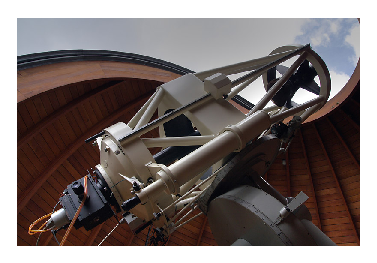
\includegraphics{./Beispiele/0,6m_telescope_in_Ostrowik_2.eps}
		}
\end{figure}
\end{frame}

\begin{frame}
\begin{figure}[h]
	\centering
		\resizebox{.5\linewidth}{!}{
			\includegraphics{./Beispiele/Effelsberg_total2.eps}
		}
\end{figure}
\end{frame}

\begin{frame}
\begin{figure}[h]
	\centering
		\resizebox{.5\linewidth}{!}{
			\includegraphics{./Beispiele/Solar_troughs_in_the_Negev_desert_of_Israel.eps}
		}
\end{figure}
\end{frame}

\subsection{Übersicht}
\begin{frame}
\begin{itemize}
	\item {\it Kreis}
	\item Ellipse
	\item Parabel
	\item Hyperbel
\end{itemize}
\end{frame}

\begin{frame}
\centerline{\huge Demo}
\end{frame}

\section{Abstrakt-Geometrische Herangehensweise}
\subsection{Vorraussetzungen}
\begin{frame}
\begin{definition}
	$\text{$K$: }x^2+y^2=\frac{z^2}{m^2} \text{ mit } x,y,z\in \mathbb{R};m\in \mathbb{R}$
\end{definition}
\end{frame}

\begin{frame}
\begin{definition}
	$\text{$E$: }0=ax+by+cz+t$ \\
	mit $x,y,z\in \mathbb{R}; a,b,c,t\in \mathbb{R}|(a \lor b \lor c) \neq 0$\\
	und $(0,0,0) \notin E$
\end{definition}
\end{frame}

\subsection{Demo}
\begin{frame}
\centerline{\huge Demo}
\end{frame}

\subsection{Befunde}
\begin{frame}
\begin{displaymath}
   \text{Ausprägung($v$)} = \left\{
     \begin{array}{lr}
       Kreis & E \parallel \text{Grundfläche($K$)} \wedge v < 0 \\
       Ellipse & v < 0\\
       Parabel & v = 0\\
       Hyperbel & v > 0
     \end{array}
   \right.
\end{displaymath}
\end{frame}

\section{Konstruktion}
\subsection{Definitionen}
\begin{frame}
\begin{displaymath}
	\begin{array}{rcl}
		Ellipse  & = & \{P\in E^2\;|\;\overline{{PF}_1} + \overline{{PF}_2} = 2a\}\\
		Parabel  & = & \{P\in E^2\;|\;\overline{PF} = \overline{Pl}\}\\
		Hyperbel & = & \{P\in E^2\;|\;|\overline{{PF}_2} - \overline{{PF}_1}| = 2a\}
	\end{array}
\end{displaymath}
\end{frame}

\subsection{Ellipse}
\begin{frame}
\begin{figure}[h]
	\centering
		\resizebox{.5\linewidth}{!}{
			\begin{pspicture}(-6,-4)(6,4)
	\psgrid[griddots=3, subgriddiv=0]
	\psellipse[linewidth=2pt](0, 0)(5.035,3.035)
	\uput*[270](0,0){$M$}
	\uput*[310](2.5,-2.6){$P$}
	\uput*[60](4,0){${F}_1$}
	\uput*[180](-4,0){${F}_2$}
	\uput*[0](5,0){${S}_1$}
	\uput*[180](-5,0){${S}_2$}
	\uput*[90](0,3){${S}_3$}
	\uput*[270](0,-3){${S}_4$}
	\uput*[270](2.5,0){$a$}
	\uput*[180](0,1.5){$b$}
	\uput*[90](-2,0){$e$}
	\rput[b]{36.87}(-2,1.5){\uput[d](0,0){$a$}}
	\rput[b]{-36.87}(2,1.5){\uput[u](0,0){$a$}}
	\psline(0,0)(5,0)%a
	\psline(0,0)(0,3)%b
	\psline(0,0)(-4,0)%e
	\psline(0,3)(4,0)%S3F1
	\psline(0,3)(-4,0)%S3F2
	\psline(2.5,-2.6)(4,0)%PF1
	\psline(2.5,-2.6)(-4,0)%PF2
	\psdots[linecolor=blue](0,0)%M
	\psdots[linecolor=blue](2.5,-2.6)%P
	\psdots[linecolor=blue](4,0)%F1
	\psdots[linecolor=blue](-4,0)%F2
	\psdots[linecolor=blue](5,0)%S1
	\psdots[linecolor=blue](-5,0)%S2
	\psdots[linecolor=blue](0,3)%S3
	\psdots[linecolor=blue](0,-3)%S4
\end{pspicture}
		}
\end{figure}
\begin{displaymath}
	\begin{array}{rcl}
		Ellipse  & = & \{P\in E^2\;|\;\overline{{PF}_1} + \overline{{PF}_2} = 2a\}
	\end{array}
\end{displaymath}
\end{frame}
\begin{frame}
\centerline{\huge Demo}
\end{frame}

\subsection{Parabel}
\begin{frame}
\begin{figure}[h]
	\centering
		\resizebox{.5\linewidth}{!}{
			\begin{pspicture}(-3,-4)(5,4)
	\psgrid[griddots=3, subgriddiv=0]
	\rput{90}(4,-4){\parabola[linewidth=2pt](0,0)(4,4)}
	\pscircle[linestyle=dashed](1,0){3}
	\uput*[143](0,0){$S$}
	\uput*[0](1,0){$F$}
	\uput*[180](-1,0){$F'$}
	\uput*[0](2,0){$D$}
	\uput[240](2,-2.83){$P$}
	\uput{.3}[245](2,2.83){$P'$}
	\uput*[180](-1,3.5){$l$}
	\uput*[180](2,3.5){$d$}
	\uput[40](0,0){$p$}
	\psline(-1,-4)(-1,4)%l
	\psline[linestyle=dashed](2,-4)(2,4)%d
	\psline(-1,0)(1,0)%p
	\psline(1,0)(2,-2.83)%PF
	\psline(-1,-2.83)(2,-2.83)%Pl
	\psdots[linecolor=blue](0,0)%S
	\psdots[linecolor=blue](1,0)%F
	\psdots[linecolor=blue](-1,0)%F'
	\psdots[linecolor=blue](2,0)%D
	\psdots[linecolor=blue](2,-2.83)%P
	\psdots[linecolor=blue](2,2.83)%P'
\end{pspicture}
		}
\end{figure}
\begin{displaymath}
	\begin{array}{rcl}
		Parabel  & = & \{P\in E^2\;|\;\overline{PF} = \overline{Pl}\}\
	\end{array}
\end{displaymath}
\end{frame}
\begin{frame}
\centerline{\huge Demo}
\end{frame}

\subsection{Hyperbel}
\begin{frame}
\begin{figure}[h]
	\centering
		\resizebox{.5\linewidth}{!}{
			\begin{pspicture}(-5,-4)(5,4)
	\psset{algebraic,plotpoints=500}
	\psgrid[griddots=3, subgriddiv=0]
	\psplot[linewidth=2pt]{1}{4.123}{sqrt(x^2-1)}
	\psplot[linewidth=2pt]{1}{4.123}{-sqrt(x^2-1)}
	\psplot[linewidth=2pt]{-1}{-4.123}{sqrt(x^2-1)}
	\psplot[linewidth=2pt]{-1}{-4.123}{-sqrt(x^2-1)}
	\pscircle[linestyle=dashed](1.4142,0){1}
	\pscircle[linestyle=dashed](-1.4142,0){1}
	\pscircle[linestyle=dashed](1.4142,0){3}
	\pscircle[linestyle=dashed](-1.4142,0){3}
	\uput*[270](0,0){$M$}
	\uput{0.3}[20](1.4142,1){$P$}
	\uput{0.3}[340](1.4142,-1){$P'$}
	\uput{0.3}[160](-1.4142,1){$P''$}
	\uput{0.3}[200](-1.4142,-1){$P'''$}
	\uput*{0.1}[0](1.4142,0){${F}_1$}
	\uput*[180](-1.4142,0){${F}_2$}
	\uput[240](1,0){${S}_1$}
	\uput[300](-1,0){${S}_2$}
	\uput*[0](2,0){$D$}
	\uput*[90](0.5,0){$a$}
	\uput*[150](0,0.5){$b$}
	\uput*{0.04}[90](-0.7071,0){$e$}
	\psline(0,0)(1,0)%a
	\psline(0,0)(0,1)%b
	\psline(0,0)(-1.4142,0)%e
	\psline(1.4142,1)(1.4142,0)%PF1
	\psline(1.4142,1)(-1.4142,0)%PF2
	\psdots[linecolor=blue](0,0)%M
	\psdots[linecolor=blue](1,0)%S1
	\psdots[linecolor=blue](-1,0)%S2
	\psdots[linecolor=blue](1.4142,0)%F1
	\psdots[linecolor=blue](-1.4142,0)%F2
	\psdots[linecolor=blue](2,0)%D
	\psdots[linecolor=blue](1.4142,1)%P
	\psdots[linecolor=blue](1.4142,-1)%P'
	\psdots[linecolor=blue](-1.4142,1)%P''
	\psdots[linecolor=blue](-1.4142,-1)%P'''
\end{pspicture}
		}
\end{figure}
\begin{displaymath}
	\begin{array}{rcl}
		Hyperbel & = & \{P\in E^2\;|\;|\overline{{PF}_2} - \overline{{PF}_1}| = 2a\}
	\end{array}
\end{displaymath}
\end{frame}
\begin{frame}
\centerline{\huge Demo}
\end{frame}

\section{Formale Beschreibung}
\subsection{Exzentrität}
\begin{frame}
\frametitle{Lineare Exzentrität}
\begin{definition}
	$e = \sqrt{a^2\pm b^2}$
\end{definition}
\end{frame}

\begin{frame}
\begin{figure}[h]
	\centering
		\resizebox{.5\linewidth}{!}{
			\begin{pspicture}(-6,-4)(6,4)
	\psgrid[griddots=3, subgriddiv=0]
	\psellipse[linewidth=2pt](0, 0)(5.035,3.035)
	\uput*[270](0,0){$M$}
	\uput*[310](2.5,-2.6){$P$}
	\uput*[60](4,0){${F}_1$}
	\uput*[180](-4,0){${F}_2$}
	\uput*[0](5,0){${S}_1$}
	\uput*[180](-5,0){${S}_2$}
	\uput*[90](0,3){${S}_3$}
	\uput*[270](0,-3){${S}_4$}
	\uput*[270](2.5,0){$a$}
	\uput*[180](0,1.5){$b$}
	\uput*[90](-2,0){$e$}
	\rput[b]{36.87}(-2,1.5){\uput[d](0,0){$a$}}
	\rput[b]{-36.87}(2,1.5){\uput[u](0,0){$a$}}
	\psline(0,0)(5,0)%a
	\psline(0,0)(0,3)%b
	\psline(0,0)(-4,0)%e
	\psline(0,3)(4,0)%S3F1
	\psline(0,3)(-4,0)%S3F2
	\psline(2.5,-2.6)(4,0)%PF1
	\psline(2.5,-2.6)(-4,0)%PF2
	\psdots[linecolor=blue](0,0)%M
	\psdots[linecolor=blue](2.5,-2.6)%P
	\psdots[linecolor=blue](4,0)%F1
	\psdots[linecolor=blue](-4,0)%F2
	\psdots[linecolor=blue](5,0)%S1
	\psdots[linecolor=blue](-5,0)%S2
	\psdots[linecolor=blue](0,3)%S3
	\psdots[linecolor=blue](0,-3)%S4
\end{pspicture}
		}
\end{figure}
\begin{displaymath}
	\begin{array}{ccccll}
		\overline{M{F}_1}^2 & + & \overline{M{S}_3}^2 & = & \overline{{F}_1{S}_3}^2 &\\
		e^2 & + & b^2 & = & a^2 &\\
		&& e & = & \sqrt{a^2-b^2}
	\end{array}
\end{displaymath}
\end{frame}

\begin{frame}
\begin{figure}[h]
	\centering
		\resizebox{.5\linewidth}{!}{
			\begin{pspicture}(-5,-4)(5,4)
	\psset{algebraic,plotpoints=500}
	\psgrid[griddots=3, subgriddiv=0]
	\psplot[linewidth=2pt]{1}{4.123}{sqrt(x^2-1)}
	\psplot[linewidth=2pt]{1}{4.123}{-sqrt(x^2-1)}
	\psplot[linewidth=2pt]{-1}{-4.123}{sqrt(x^2-1)}
	\psplot[linewidth=2pt]{-1}{-4.123}{-sqrt(x^2-1)}
	\pscircle[linestyle=dashed](1.4142,0){1}
	\pscircle[linestyle=dashed](-1.4142,0){1}
	\pscircle[linestyle=dashed](1.4142,0){3}
	\pscircle[linestyle=dashed](-1.4142,0){3}
	\uput*[270](0,0){$M$}
	\uput{0.3}[20](1.4142,1){$P$}
	\uput{0.3}[340](1.4142,-1){$P'$}
	\uput{0.3}[160](-1.4142,1){$P''$}
	\uput{0.3}[200](-1.4142,-1){$P'''$}
	\uput*{0.1}[0](1.4142,0){${F}_1$}
	\uput*[180](-1.4142,0){${F}_2$}
	\uput[240](1,0){${S}_1$}
	\uput[300](-1,0){${S}_2$}
	\uput*[0](2,0){$D$}
	\uput*[90](0.5,0){$a$}
	\uput*[150](0,0.5){$b$}
	\uput*{0.04}[90](-0.7071,0){$e$}
	\psline(0,0)(1,0)%a
	\psline(0,0)(0,1)%b
	\psline(0,0)(-1.4142,0)%e
	\psline(1.4142,1)(1.4142,0)%PF1
	\psline(1.4142,1)(-1.4142,0)%PF2
	\psdots[linecolor=blue](0,0)%M
	\psdots[linecolor=blue](1,0)%S1
	\psdots[linecolor=blue](-1,0)%S2
	\psdots[linecolor=blue](1.4142,0)%F1
	\psdots[linecolor=blue](-1.4142,0)%F2
	\psdots[linecolor=blue](2,0)%D
	\psdots[linecolor=blue](1.4142,1)%P
	\psdots[linecolor=blue](1.4142,-1)%P'
	\psdots[linecolor=blue](-1.4142,1)%P''
	\psdots[linecolor=blue](-1.4142,-1)%P'''
\end{pspicture}
		}
\end{figure}
\begin{displaymath}
	\begin{array}{ccccll}
		\overline{M{S}_1}^2 & + & \overline{{S}_1{F'}_1}^2 & = & \overline{M{F'}_1}^2 &\\
		a^2 & + & b^2 & = & e^2 &\\
		&& e & = & \sqrt{a^2+b^2}
	\end{array}
\end{displaymath}
\end{frame}

\begin{frame}
\frametitle{Numerische Exzentrität}
\begin{definition}
	$\epsilon = \frac{e}{a}$
\end{definition}
\end{frame}

\begin{frame}
\begin{displaymath}
   \text{Ausprägung($\epsilon$)} = \left\{
     \begin{array}{lr}
       Kreis & \epsilon = 0 \\
       Ellipse & \epsilon < 1\\
       Parabel & \epsilon = 1\\
       Hyperbel & \epsilon > 1
     \end{array}
   \right.
\end{displaymath}
\end{frame}

\subsection{Ellipse}
\begin{frame}
\begin{figure}[h]
	\centering
		\resizebox{.5\linewidth}{!}{
			\begin{pspicture}(-6,-4)(6,4)
	\psgrid[griddots=3, subgriddiv=0]
	\psellipse[linewidth=2pt](0, 0)(5.035,3.035)
	\uput*[270](0,0){$M$}
	\uput*[310](2.5,-2.6){$P$}
	\uput*[60](4,0){${F}_1$}
	\uput*[180](-4,0){${F}_2$}
	\uput*[0](5,0){${S}_1$}
	\uput*[180](-5,0){${S}_2$}
	\uput*[90](0,3){${S}_3$}
	\uput*[270](0,-3){${S}_4$}
	\uput*[270](2.5,0){$a$}
	\uput*[180](0,1.5){$b$}
	\uput*[90](-2,0){$e$}
	\rput[b]{36.87}(-2,1.5){\uput[d](0,0){$a$}}
	\rput[b]{-36.87}(2,1.5){\uput[u](0,0){$a$}}
	\psline(0,0)(5,0)%a
	\psline(0,0)(0,3)%b
	\psline(0,0)(-4,0)%e
	\psline(0,3)(4,0)%S3F1
	\psline(0,3)(-4,0)%S3F2
	\psline(2.5,-2.6)(4,0)%PF1
	\psline(2.5,-2.6)(-4,0)%PF2
	\psdots[linecolor=blue](0,0)%M
	\psdots[linecolor=blue](2.5,-2.6)%P
	\psdots[linecolor=blue](4,0)%F1
	\psdots[linecolor=blue](-4,0)%F2
	\psdots[linecolor=blue](5,0)%S1
	\psdots[linecolor=blue](-5,0)%S2
	\psdots[linecolor=blue](0,3)%S3
	\psdots[linecolor=blue](0,-3)%S4
\end{pspicture}
		}
\end{figure}
\begin{displaymath}
	\begin{array}{rcl}
		\overline{{PF}_1} + \overline{{PF}_2} & = & 2a\\
		\sqrt{{(e+x)}^2 + y^2} + \sqrt{{(e-x)}^2 + y^2} & = & 2a
	\end{array}
\end{displaymath}
\end{frame}

\begin{frame}
\begin{displaymath}
	\begin{array}{rcl}
		\overline{{PF}_1} + \overline{{PF}_2} & = & 2a\\
		\sqrt{{(e+x)}^2 + y^2} + \sqrt{{(e-x)}^2 + y^2} & = & 2a\\
		\sqrt{{(e+x)}^2 + y^2} & = & 2a - \sqrt{{(e-x)}^2 + y^2}\\
		\sqrt{{(e+x)}^2 + y^2}^2 & = & \left (2a - \sqrt{{(e-x)}^2 + y^2}\right )^2\\
		e^2 + 2ex + x^2 + y^2 & = & 4a^2 - 4a \sqrt{(e-x)^2+y^2}\\
		&& + e^2 - 2ex + x^2 + y^2\\
		a\sqrt{{(e-x)}^2 + y^2} & = & a^2 - ex\\
	\end{array}
\end{displaymath}
\end{frame}

\begin{frame}
\begin{displaymath}
	\begin{array}{rcl}
		\left (a\sqrt{{(e-x)}^2 + y^2}\right )^2 & = & \left(a^2 - ex\right)^2\\
		a^2e^2 - 2a^2ex + a^2x^2 + a^2y^2 &=& a^4 - 2a^2ex + e^2x^2\\
		a^2x^2 - e^2x^2 + a^2y^2 &=& a^4 - a^2e^2\\
		\mathbf{\left(a^2 - e^2\right)}x^2 + a^2y^2 &=& a^2\mathbf{\left(a^2 - e^2\right)}\\
		\mathbf{b^2}x^2 + a^2y^2 &=& a^2\mathbf{b^2}\\
		\frac{x^2}{a^2} + \frac{y^2}{b^2} &=& 1
	\end{array}
\end{displaymath}
\end{frame}

\begin{frame}
\begin{displaymath}
	\begin{array}{rcl}
		\frac{x^2}{r^2} + \frac{y^2}{r^2} &=& 1\\
		x^2 + y^2 &=& r^2
	\end{array}
\end{displaymath}
\end{frame}

\subsection{Parabel}
\begin{frame}
\begin{figure}[h]
	\centering
		\resizebox{.5\linewidth}{!}{
			\begin{pspicture}(-3,-4)(5,4)
	\psgrid[griddots=3, subgriddiv=0]
	\rput{90}(4,-4){\parabola[linewidth=2pt](0,0)(4,4)}
	\pscircle[linestyle=dashed](1,0){3}
	\uput*[143](0,0){$S$}
	\uput*[0](1,0){$F$}
	\uput*[180](-1,0){$F'$}
	\uput*[0](2,0){$D$}
	\uput[240](2,-2.83){$P$}
	\uput{.3}[245](2,2.83){$P'$}
	\uput*[180](-1,3.5){$l$}
	\uput*[180](2,3.5){$d$}
	\uput[40](0,0){$p$}
	\psline(-1,-4)(-1,4)%l
	\psline[linestyle=dashed](2,-4)(2,4)%d
	\psline(-1,0)(1,0)%p
	\psline(1,0)(2,-2.83)%PF
	\psline(-1,-2.83)(2,-2.83)%Pl
	\psdots[linecolor=blue](0,0)%S
	\psdots[linecolor=blue](1,0)%F
	\psdots[linecolor=blue](-1,0)%F'
	\psdots[linecolor=blue](2,0)%D
	\psdots[linecolor=blue](2,-2.83)%P
	\psdots[linecolor=blue](2,2.83)%P'
\end{pspicture}
		}
\end{figure}
\begin{displaymath}
	\begin{array}{rcl}
		\overline{PF} &=& \overline{Pl}\\
		\sqrt{\left(x-\frac{p}{2}\right)^2+y^2} &=& \frac{p}{2} + x\\
	\end{array}
\end{displaymath}
\end{frame}

\begin{frame}
\begin{displaymath}
	\begin{array}{rcl}
		\overline{PF} &=& \overline{Pl}\\
		\sqrt{\left(x-\frac{p}{2}\right)^2+y^2} &=& \frac{p}{2} + x\\
		\left(x-\frac{p}{2}\right)^2+y^2 &=& \left(\frac{p}{2} + x\right)^2\\
		x^2 - px + \frac{p^2}{4} + y^2 &=& x^2 + px + \frac{p^2}{4}\\
		y^2 &=& 2px
	\end{array}
\end{displaymath}
\end{frame}

\subsection{Hyperbel}
\begin{frame}
\begin{figure}[h]
	\centering
		\resizebox{.5\linewidth}{!}{
			\begin{pspicture}(-5,-4)(5,4)
	\psset{algebraic,plotpoints=500}
	\psgrid[griddots=3, subgriddiv=0]
	\psplot[linewidth=2pt]{1}{4.123}{sqrt(x^2-1)}
	\psplot[linewidth=2pt]{1}{4.123}{-sqrt(x^2-1)}
	\psplot[linewidth=2pt]{-1}{-4.123}{sqrt(x^2-1)}
	\psplot[linewidth=2pt]{-1}{-4.123}{-sqrt(x^2-1)}
	\pscircle[linestyle=dashed](1.4142,0){1}
	\pscircle[linestyle=dashed](-1.4142,0){1}
	\pscircle[linestyle=dashed](1.4142,0){3}
	\pscircle[linestyle=dashed](-1.4142,0){3}
	\uput*[270](0,0){$M$}
	\uput{0.3}[20](1.4142,1){$P$}
	\uput{0.3}[340](1.4142,-1){$P'$}
	\uput{0.3}[160](-1.4142,1){$P''$}
	\uput{0.3}[200](-1.4142,-1){$P'''$}
	\uput*{0.1}[0](1.4142,0){${F}_1$}
	\uput*[180](-1.4142,0){${F}_2$}
	\uput[240](1,0){${S}_1$}
	\uput[300](-1,0){${S}_2$}
	\uput*[0](2,0){$D$}
	\uput*[90](0.5,0){$a$}
	\uput*[150](0,0.5){$b$}
	\uput*{0.04}[90](-0.7071,0){$e$}
	\psline(0,0)(1,0)%a
	\psline(0,0)(0,1)%b
	\psline(0,0)(-1.4142,0)%e
	\psline(1.4142,1)(1.4142,0)%PF1
	\psline(1.4142,1)(-1.4142,0)%PF2
	\psdots[linecolor=blue](0,0)%M
	\psdots[linecolor=blue](1,0)%S1
	\psdots[linecolor=blue](-1,0)%S2
	\psdots[linecolor=blue](1.4142,0)%F1
	\psdots[linecolor=blue](-1.4142,0)%F2
	\psdots[linecolor=blue](2,0)%D
	\psdots[linecolor=blue](1.4142,1)%P
	\psdots[linecolor=blue](1.4142,-1)%P'
	\psdots[linecolor=blue](-1.4142,1)%P''
	\psdots[linecolor=blue](-1.4142,-1)%P'''
\end{pspicture}
		}
\end{figure}
\begin{displaymath}
	\begin{array}{rcl}
		\overline{{PF}_1} - \overline{{PF}_2} & = & 2a\\
		\sqrt{{(e+x)}^2 + y^2} - \sqrt{{(e-x)}^2 + y^2} & = & 2a\\
		\sqrt{{(e+(-x))}^2 + y^2} - \sqrt{{((-x)-e)}^2 + y^2} & = & 2a\\
	\end{array}
\end{displaymath}
\end{frame}

\begin{frame}
\begin{displaymath}
	\begin{array}{rcl}
		\overline{{PF}_1} - \overline{{PF}_2} & = & 2a\\
		\sqrt{{(e+x)}^2 + y^2} - \sqrt{{(e-x)}^2 + y^2} & = & 2a\\
		\sqrt{{(e+x)}^2 + y^2} & = & 2a + \sqrt{{(e-x)}^2 + y^2}\\
		\sqrt{{(e+x)}^2 + y^2}^2 & = & \left (2a + \sqrt{{(e-x)}^2 + y^2}\right )^2\\
		e^2 + 2ex + x^2 + y^2 & = & 4a^2 + 4a \sqrt{(e-x)^2+y^2}\\
		&& + e^2 - 2ex + x^2 + y^2\\
		a\sqrt{{(e-x)}^2 + y^2} & = & ex - a^2\\
	\end{array}
\end{displaymath}
\end{frame}

\begin{frame}
\begin{displaymath}
	\begin{array}{rcl}
		\left (a\sqrt{{(e-x)}^2 + y^2}\right )^2 & = & \left(ex - a^2\right)^2\\
		a^2e^2 - 2a^2ex + a^2x^2 + a^2y^2 &=& e^2x^2 - 2a^2ex + a^4\\
		a^2e^2 - a^4 &=& e^2x^2 - a^2x^2 - a^2y^2\\
		e^2x^2 - a^2x^2 - a^2y^2 &=& a^2e^2 - a^4\\
		\left(e^2 - a^2\right)x^2 - a^2y^2 &=& a^2\left(e^2 - a^2\right)\\
		b^2x^2 - a^2y^2 &=& a^2b^2\\
		\frac{x^2}{a^2} - \frac{y^2}{b^2} &=& 1
	\end{array}
\end{displaymath}
\end{frame}

\begin{frame}
\begin{displaymath}
	\begin{array}{rcl}
		\overline{{PF}_1} - \overline{{PF}_2} & = & 2a\\
		\sqrt{{(e+(-x))}^2 + y^2} & = & 2a\\
		- \sqrt{{((-x)-e)}^2 + y^2} &&\\
		\sqrt{{(e-x)}^2 + y^2} & = & 2a + \sqrt{{(-e-x)}^2 + y^2}\\
		\sqrt{{(e-x)}^2 + y^2}^2 & = & \left (2a + \sqrt{{(-e-x)}^2 + y^2}\right )^2\\
		e^2 - 2ex + x^2 + y^2 & = & 4a^2 + 4a \sqrt{(-e-x)^2+y^2}\\
		&& + e^2 + 2ex + x^2 + y^2\\
		a\sqrt{{(-e-x)}^2 + y^2} & = & -ex - a^2\\
	\end{array}
\end{displaymath}
\end{frame}

\begin{frame}
\begin{displaymath}
	\begin{array}{rcl}
		\left (a\sqrt{{(-e-x)}^2 + y^2}\right )^2 & = & \left(-ex - a^2\right)^2\\
		a^2e^2 + 2a^2ex + a^2x^2 + a^2y^2 &=& e^2x^2 + 2a^2ex + a^4\\
		a^2e^2 - a^4 &=& e^2x^2 - a^2x^2 - a^2y^2\\
		e^2x^2 - a^2x^2 - a^2y^2 &=& a^2e^2 - a^4\\
		\left(e^2 - a^2\right)x^2 - a^2y^2 &=& a^2\left(e^2 - a^2\right)\\
		b^2x^2 - a^2y^2 &=& a^2b^2\\
		\frac{x^2}{a^2} - \frac{y^2}{b^2} &=& 1
	\end{array}
\end{displaymath}
\end{frame}

\end{document}